\documentclass[article]{standalone}               
\usepackage{tikz,pgfplots}
\usetikzlibrary{arrows,backgrounds}
\usepgflibrary{shapes.multipart}
\pgfplotsset{compat=1.15}
\usepackage{adjustbox}
\definecolor{webgreen}{rgb}{0,.5,0}
\definecolor{webbrown}{rgb}{.6,0,0}
\definecolor{webyellow}{rgb}{0.98,0.92,0.73}
\definecolor{webgray}{rgb}{.753,.753,.753}
\definecolor{webblue}{rgb}{0,0,.8}
\definecolor{webgreen}{rgb}{0, 0.5, 0} % less intense green
\definecolor{webred}{rgb}{0.5, 0, 0}   % less intense red

		\def\constProcFreq{1}	% processor frequency, GHz
\def\constMPE{1} % If MPE trick (see Taihulight) in use
\def\constProcPerformance{(100*\constMPE)}  %processor performance, GFlops
\def\constNoOfProcessors{x*1e9/\constProcPerformance} % x in Eflop/s
\def\constTotalClocks{2e13} % Total measurement time, in ticks
\def\constContextChange{1e4} % Time of context change, in ticks


%% Derived 

%\def\constProcFreq{1}	% processor frequency, GHz
\def\constMicroSecToTicks{1e3*\constProcFreq}  % usec time to clock ticks
%\def\constNoOfProcessors{x*1e8/64}
% Calculate different \alpha contributions
\def\constAlphaContext{\constContextChange/\constTotalClocks}
\def\constAlphaLoop{\constNoOfProcessors/\constTotalClocks}
\def\constAlphaOS{\constAlphaContext
	+\constAlphaLoop
}
% The sum of all contributions
\def\constAlphaTotal{(\constAlphaSW+\constAlphaOS)}
\def\constMinusAlpha{1-\constAlphaTotal}
\def\constEfficiency{(\constNoOfProcessors*\constAlphaTotal+\constMinusAlpha)}
\def\constRMax{x/\constEfficiency}
\def\constPropagationDelay{\constNoOfProcessors*1e-6/2e-8*2e9/\constTotalClocks*1000}
\begin{document}
\begin{tabular}{cc}
		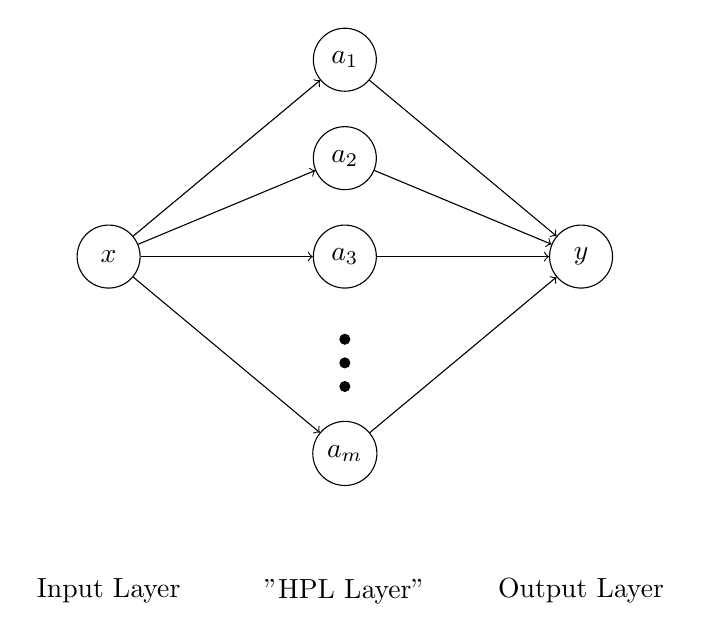
\begin{tikzpicture}
\tikzstyle{place}=[circle, draw=black, minimum size = 8mm]

% Input
\draw node at (0, -3*1.25) [place] (first_3) {$x$};
%\foreach \x in {1,...,3}

% Hidden 1
\foreach \x in {1,...,3}
\node at (3, -\x*1.25) [place] (second_\x){$a_\x$};
\foreach \x in {1,...,3}
\fill (3, -4.5 -\x*0.3) circle (2pt);
\draw node at (3, -5*1.25) [place] (second_m) {$a_m$};

%% Hidden 2
%\foreach \x in {1,...,3}
%\node at (6, -\x*1.25) [place] (third_\x){$b_\x$};
%\foreach \x in {1,...,3}
%\fill (6, -4.5 -\x*0.3) circle (2pt);
%\draw node at (6, -5*1.25) [place] (third_m) {$b_m$};
%
%% Output
%\foreach \x in {1,...,3}
%\node at (9, -\x*1.25) [place] (fourth_\x){$y_\x$};
%\foreach \x in {1,...,3}
%\fill (9, -4.5 -\x*0.3) circle (2pt);
%\node at (9, -5*1.25) [place] (fourth_m) {$y_k$};
% Input
\draw node at (6, -3*1.25) [place] (fourth_3) {$y$};
%\foreach \x in {1,...,3}
%
%% Input -> Hidden1
%\foreach \i in {1,...,3}
\foreach \j in {1,...,3}
\draw [->] (first_3) to (second_\j);
%\foreach \i in {1,...,3}
%\draw [->] (first_\i) to (second_m);
%\foreach \i in {1,...,3}
%\draw [->] (first_n) to (second_\i);
\draw [->] (first_3) to (second_m);
%
%% Hidden1 -> Hidden2
%\foreach \i in {1,...,3}
%\foreach \j in {1,...,3}
%\draw [->] (second_\i) to (fourth_3);
%\foreach \i in {1,...,3}
%\draw [->] (second_\i) to (fourth_m);
%\foreach \i in {1,...,3}
%\draw [->] (second_m) to (third_\i);
%\draw [->] (second_m) to (third_m);
%
%% Hidden -> Output
%\foreach \i in {1,...,3}
\foreach \j in {1,...,3}
\draw [->] (second_\j) to (fourth_3);
%\foreach \i in {1,...,3}
%\draw [->] (third_\i) to (fourth_m);
\draw [->] (second_m) to (fourth_3);
%
%% Text
\node at (0, -8) [black, ] {Input Layer};
\node at (3, -8) [black, ] {"HPL Layer"};
%\node at (6, -8) [black, ] {Hidden Layer2};
\node at (6, -8) [black, ] {Output Layer};
\end{tikzpicture}
	&
	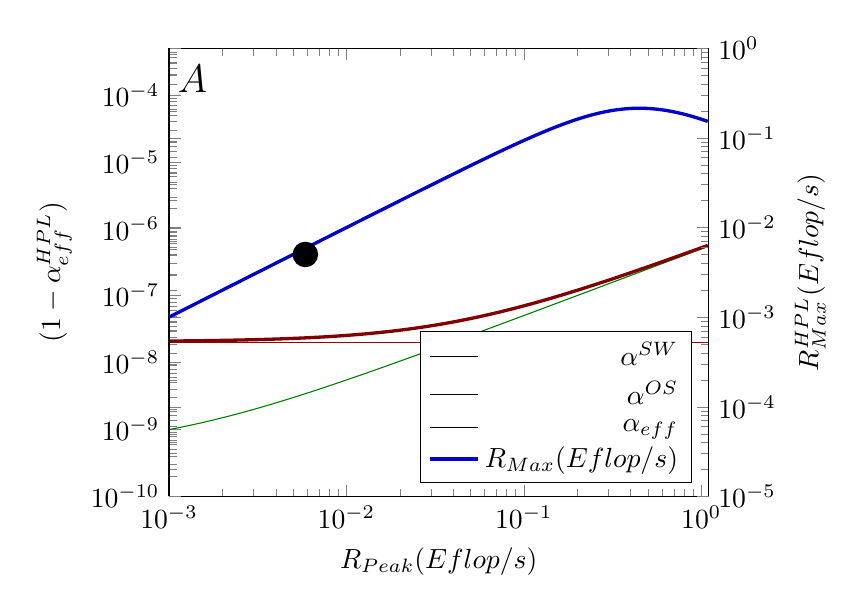
\begin{tikzpicture}
	
	\def\constAlphaSW{2e-8}
	
	\pgfplotsset{
		%    scale only axis,
		%    scaled x ticks=base 10:3,
		xmin=0.001, xmax=1.1,
	}
	
	\begin{axis}[
	axis y line*=left,
	legend style={
		cells={anchor=east},
		legend pos={north west},
	},
	xlabel=$R_{Peak}(Eflop/s)$,
	ylabel=$(1-\alpha_{eff}^{HPL})$,
	ymin=1e-10, ymax=5e-4,
	xmode=log,
	log basis x=10,
	ymode=log,
	log basis y=10,
	]
	% The SW contribution is constant
	\addplot[samples=501,domain=.001:1.1,webbrown]
	{\constAlphaSW }; \label{plot_SW}
	
	% Now calculate contribution of the OS
	\addplot[samples=501,domain=.001:1.1,webgreen]
	{\constAlphaOS} ;\label{plot_loop}
	
	%% Calculate propagation delay
	%\addplot[samples=501,domain=.001:1.1,webyellow]
	%{\constPropagationDelay} ;\label{plot_delay}
	%
	% Calculate total alpha 
	\addplot[samples=501,domain=.001:1.1,webred,very thick]
	{\constAlphaTotal} ;\label{plot_total}
	
	\end{axis}
	
	\begin{axis}[
	%  axis y line*=right,
	ylabel near ticks, yticklabel pos=right,
	axis x line=none,
	ymin=0.00001, ymax=1.0,
	xmode=log,
	log basis x=10,
	ymode=log,
	log basis y=10,
	ylabel=$R_{Max}^{HPL}(Eflop/s)$,
	legend style={
		cells={anchor=east},
		legend pos={south east},
	},
	]
	\addlegendimage{/pgfplots/refstyle=plot_SW}
	\addlegendentry{$\alpha^{SW}$}
	\addlegendimage{/pgfplots/refstyle=plot_loop}
	\addlegendentry{$\alpha^{OS}$}
	%\addlegendimage{/pgfplots/refstyle=plot_delay}
	%\addlegendentry{$\alpha^{delay}$}
	\addlegendimage{/pgfplots/refstyle=plot_total}
	\addlegendentry{$\alpha_{eff}$}
	%
	%%% Calculate efficiency
	%\addplot[samples=501,domain=.001:1.1,webblue] 
	%{\constRMax/x};\label{plot_eff}
	
	%% Calculate Rmax
	\addplot[samples=501,domain=.001:1.1,webblue,very thick] 
	{\constRMax};\label{plot_rmax}
	
	%\addlegendimage{/pgfplots/refstyle=plot_eff}
	%\addlegendentry{$Efficiency$}
	\addlegendimage{/pgfplots/refstyle=plot_rmax}
	\addlegendentry{$R_{Max}(Eflop/s)$}
	\addplot[only marks,  mark=*,  mark size=4, very thick] plot coordinates {
		(0.00587,0.005) %JUQUEEN computer at HPL
	};
	
	\end{axis}
	\draw node at (0.3, 5.3)  (A) {\Large $A$};
	
	\end{tikzpicture}
	
	\\	
		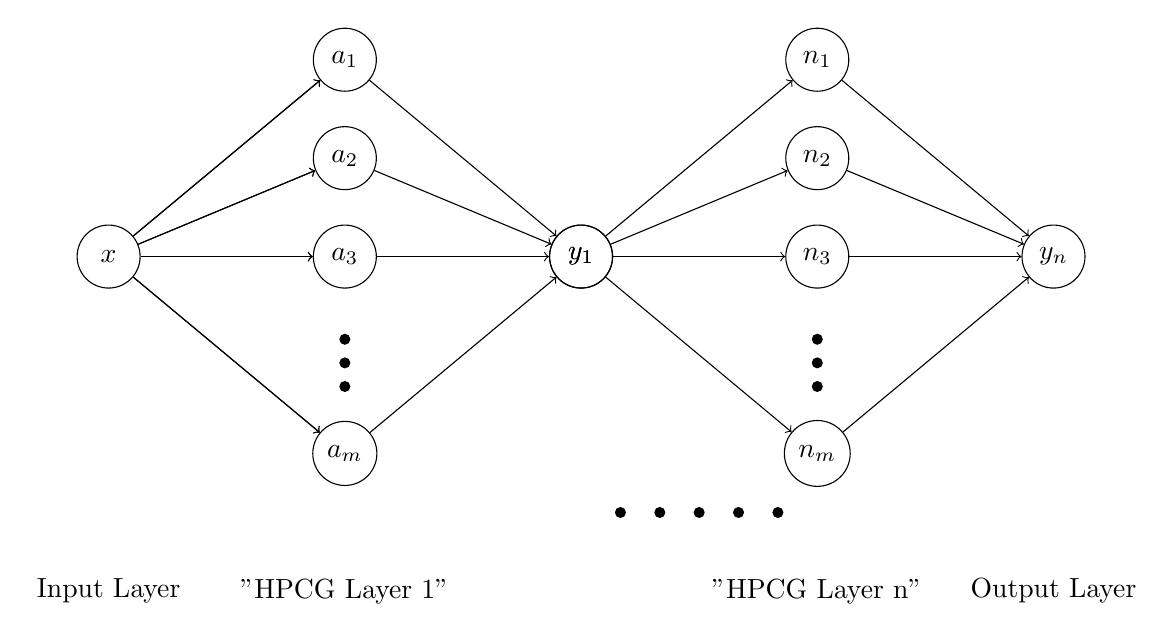
\begin{tikzpicture}
\tikzstyle{place}=[circle, draw=black, minimum size = 8mm]

% Input
\draw node at (0, -3*1.25) [place] (first_3) {$x$};
%\foreach \x in {1,...,3}

% Hidden 1
\foreach \x in {1,...,3}
\node at (3, -\x*1.25) [place] (second_\x){$a_\x$};
\foreach \x in {1,...,3}
\fill (3, -4.5 -\x*0.3) circle (2pt);
\draw node at (3, -5*1.25) [place] (second_m) {$a_m$};

%% Hidden 2
%\foreach \x in {1,...,3}
%\node at (6, -\x*1.25) [place] (third_\x){$b_\x$};
%\foreach \x in {1,...,3}
%\fill (6, -4.5 -\x*0.3) circle (2pt);
%\draw node at (6, -5*1.25) [place] (third_m) {$b_m$};
%
%% Output
%\foreach \x in {1,...,3}
%\node at (9, -\x*1.25) [place] (fourth_\x){$y_\x$};
%\foreach \x in {1,...,3}
%\fill (9, -4.5 -\x*0.3) circle (2pt);
%\node at (9, -5*1.25) [place] (fourth_m) {$y_k$};
% Input
\draw node at (6, -3*1.25) [place] (y_1) {$y_1$};
\draw node at (12, -3*1.25) [place] (fourth_3) {$y_n$};
%\foreach \x in {1,...,3}
%
%% Input -> HPCG1
%\foreach \i in {1,...,3}
\foreach \j in {1,...,3}
\draw [->] (first_3) to (second_\j);
%\foreach \i in {1,...,3}
%\draw [->] (first_\i) to (second_m);
%\foreach \i in {1,...,3}
%\draw [->] (first_n) to (second_\i);
\draw [->] (first_3) to (second_m);

\draw node at (6, -3*1.25) [place] (y_1) {$y_1$};
\foreach \j in {1,...,3}
\draw [->] (second_\j) to (y_1);
\draw [->] (second_m) to (y_1);


%% HPCG1 -> HPCGn
%\foreach \i in {1,...,3}
\foreach \j in {1,...,3}
\draw [->] (first_3) to (second_\j);
%\foreach \i in {1,...,3}
%\draw [->] (first_\i) to (second_m);
%\foreach \i in {1,...,3}
%\draw [->] (first_n) to (second_\i);
\draw [->] (first_3) to (second_m);
%

% Hidden 2
\foreach \x in {1,...,3}
\node at (9, -\x*1.25) [place] (third_\x){$n_\x$};
\foreach \x in {1,...,3}
\fill (9, -4.5 -\x*0.3) circle (2pt);
\draw node at (9, -5*1.25) [place] (third_m) {$n_m$};

\foreach \j in {1,...,3}
\draw [->] (y_1) to (third_\j);
\draw [->]  (y_1) to (third_m);


\foreach \y in {1,...,5}
\fill (6+\y/2, -7 ) circle (2pt);
%
%% Hidden1 -> Hidden2
%\foreach \i in {1,...,3}
%\foreach \j in {1,...,3}
%\draw [->] (second_\i) to (fourth_3);
%\foreach \i in {1,...,3}
%\draw [->] (second_\i) to (fourth_m);
%\foreach \i in {1,...,3}
%\draw [->] (second_m) to (third_\i);
%\draw [->] (second_m) to (third_m);
%
%% Hidden -> Output
%\foreach \i in {1,...,3}
\foreach \j in {1,...,3}
\draw [->] (third_\j) to (fourth_3);
%\foreach \i in {1,...,3}
%\draw [->] (third_\i) to (fourth_m);
\draw [->] (third_m) to (fourth_3);
%
%% Text
\node at (0, -8) [black, ] {Input Layer};
\node at (3, -8) [black, ] {"HPCG Layer 1"};
%\node at (6, -8) [black, ] {Hidden Layer2};
\node at (9, -8) [black, ] {"HPCG Layer n"};
\node at (12, -8) [black, ] {Output Layer};
\end{tikzpicture}
	&	
	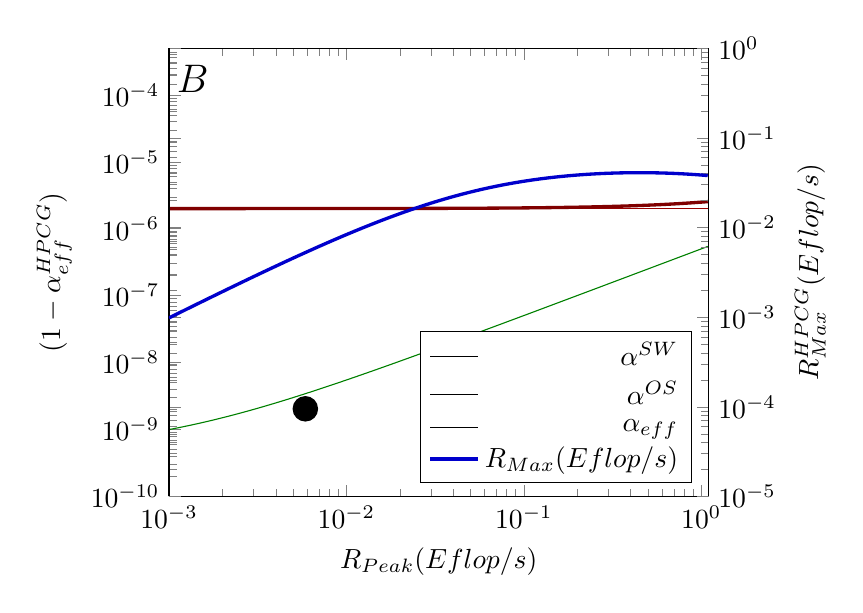
\begin{tikzpicture}
	
	\def\constAlphaSW{2e-6}
	
	\pgfplotsset{
		%    scale only axis,
		%    scaled x ticks=base 10:3,
		xmin=0.001, xmax=1.1,
	}
	
	\begin{axis}[
	axis y line*=left,
	xlabel=$R_{Peak}(Eflop/s)$,
	ylabel=$(1-\alpha_{eff}^{HPCG})$,
	ymin=1e-10, ymax=5e-4,
	xmode=log,
	log basis x=10,
	ymode=log,
	log basis y=10,
	]
	% The SW contribution is constant
	\addplot[samples=501,domain=.001:1.1,webbrown]
	{\constAlphaSW }; \label{plot_SW}
	
	% Now calculate contribution of the OS
	\addplot[samples=501,domain=.001:1.1,webgreen]
	{\constAlphaOS} ;\label{plot_loop}
	
	%% Calculate propagation delay
	%\addplot[samples=501,domain=.001:1.1,webyellow]
	%{\constPropagationDelay} ;\label{plot_delay}
	%
	% Calculate total alpha 
	\addplot[samples=501,domain=.001:1.1,webred,very thick]
	{\constAlphaTotal} ;\label{plot_total}
	
	\end{axis}
	
	\begin{axis}[
	%  axis y line*=right,
	ylabel near ticks, yticklabel pos=right,
	axis x line=none,
	ymin=0.00001, ymax=1.0,
	xmode=log,
	log basis x=10,
	ymode=log,
	log basis y=10,
	ylabel=$R_{Max}^{HPCG}(Eflop/s)$,
	legend style={
		cells={anchor=east},
		legend pos={south east},
	},
	]
	\addlegendimage{/pgfplots/refstyle=plot_SW}
	\addlegendentry{$\alpha^{SW}$}
	\addlegendimage{/pgfplots/refstyle=plot_loop}
	\addlegendentry{$\alpha^{OS}$}
	%\addlegendimage{/pgfplots/refstyle=plot_delay}
	%\addlegendentry{$\alpha^{delay}$}
	\addlegendimage{/pgfplots/refstyle=plot_total}
	\addlegendentry{$\alpha_{eff}$}
	%
	%%%% Calculate efficiency
	%\addplot[samples=501,domain=.001:1.1,webblue] 
	%{\constRMax/x};\label{plot_eff}
	
	%% Calculate Rmax
	\addplot[samples=501,domain=.001:1.1,webblue,very thick] 
	{\constRMax};\label{plot_rmax}
	
	%\addlegendimage{/pgfplots/refstyle=plot_eff}
	%\addlegendentry{$Efficiency$}
	\addlegendimage{/pgfplots/refstyle=plot_rmax}
	\addlegendentry{$R_{Max}(Eflop/s)$}
	\addplot[only marks,  mark=*,  mark size=4, very thick] plot coordinates {
		(0.00587,0.000095) %JUQUEEN computer at HPCG
	};
	
	\end{axis}
	\draw node at (0.3, 5.3)  (B) {\Large $B$};
	
	\end{tikzpicture}
	
	\\
		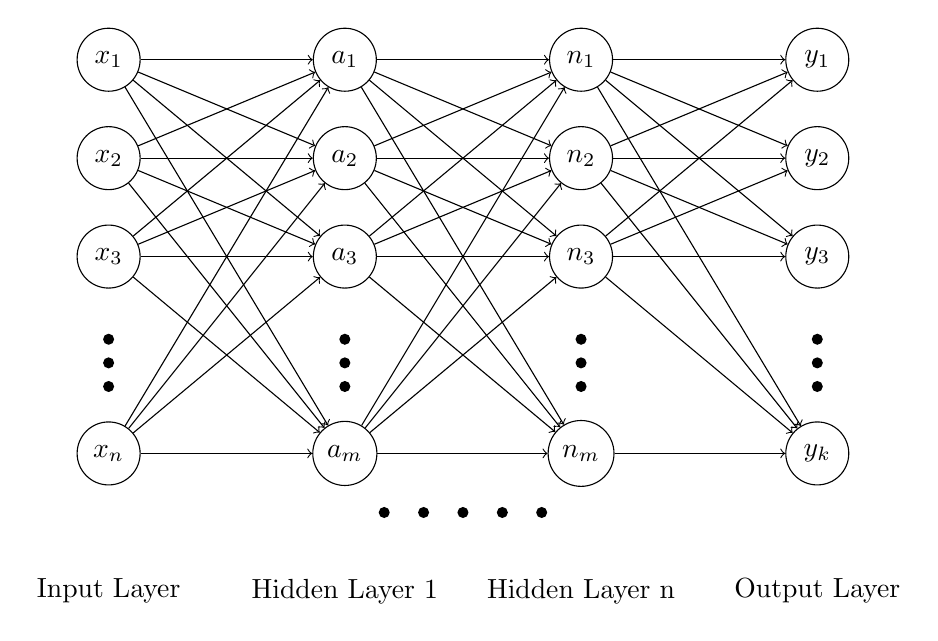
\begin{tikzpicture}
\tikzstyle{place}=[circle, draw=black, minimum size = 8mm]

% Input
\foreach \x in {1,...,3}
\draw node at (0, -\x*1.25) [place] (first_\x) {$x_\x$};
\foreach \x in {1,...,3}
\fill (0, -4.5 -\x*0.3) circle (2pt);
\draw node at (0, -5*1.25) [place] (first_n) {$x_n$};

% Hidden 1
\foreach \x in {1,...,3}
\node at (3, -\x*1.25) [place] (second_\x){$a_\x$};
\foreach \x in {1,...,3}
\fill (3, -4.5 -\x*0.3) circle (2pt);
\draw node at (3, -5*1.25) [place] (second_m) {$a_m$};

% Hidden 2
\foreach \x in {1,...,3}
\node at (6, -\x*1.25) [place] (third_\x){$n_\x$};
\foreach \x in {1,...,3}
\fill (6, -4.5 -\x*0.3) circle (2pt);
\draw node at (6, -5*1.25) [place] (third_m) {$n_m$};

% Output
\foreach \x in {1,...,3}
\node at (9, -\x*1.25) [place] (fourth_\x){$y_\x$};
\foreach \x in {1,...,3}
\fill (9, -4.5 -\x*0.3) circle (2pt);
\node at (9, -5*1.25) [place] (fourth_m) {$y_k$};

% Input -> Hidden1
\foreach \i in {1,...,3}
\foreach \j in {1,...,3}
\draw [->] (first_\i) to (second_\j);
\foreach \i in {1,...,3}
\draw [->] (first_\i) to (second_m);
\foreach \i in {1,...,3}
\draw [->] (first_n) to (second_\i);
\draw [->] (first_n) to (second_m);

% Hidden1 -> Hidden2
\foreach \i in {1,...,3}
\foreach \j in {1,...,3}
\draw [->] (second_\i) to (third_\j);
\foreach \i in {1,...,3}
\draw [->] (second_\i) to (third_m);
\foreach \i in {1,...,3}
\draw [->] (second_m) to (third_\i);
\draw [->] (second_m) to (third_m);

% Hidden -> Output
\foreach \i in {1,...,3}
\foreach \j in {1,...,3}
\draw [->] (third_\i) to (fourth_\j);
\foreach \i in {1,...,3}
\draw [->] (third_\i) to (fourth_m);
\draw [->] (third_m) to (fourth_m);

\foreach \y in {1,...,5}
\fill (3+\y/2, -7 ) circle (2pt);

% Text
\node at (0, -8) [black, ] {Input Layer};
\node at (3, -8) [black, ] {Hidden Layer 1};
\node at (6, -8) [black, ] {Hidden Layer n};
\node at (9, -8) [black, ] {Output Layer};
\end{tikzpicture}
	&
	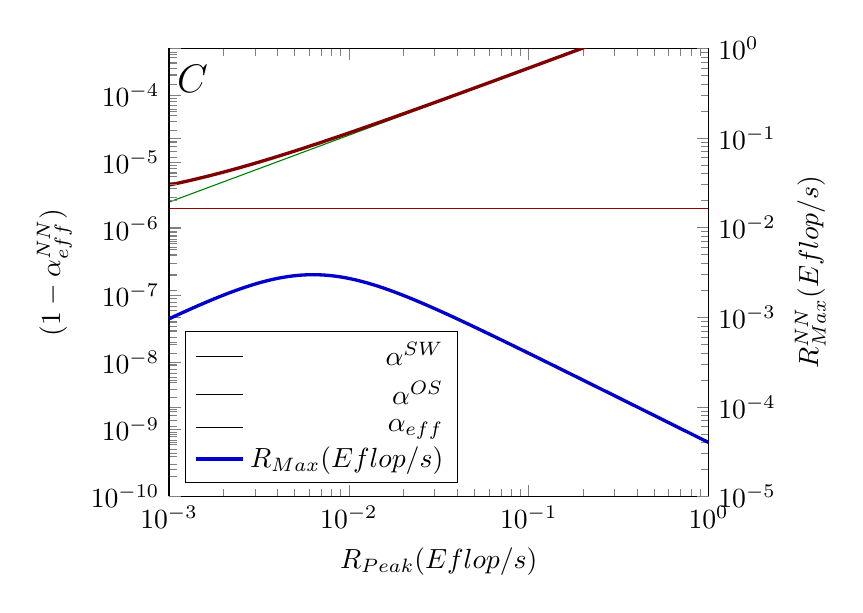
\begin{tikzpicture}
	
	\def\constAlphaSW{2e-6}
	\def\constAlphaLoop{5000*\constNoOfProcessors/\constTotalClocks}
	
	\pgfplotsset{
		%    scale only axis,
		%    scaled x ticks=base 10:3,
		xmin=0.001, xmax=1.0,
	}
	
	\begin{axis}[
	axis y line*=left,
	xlabel=$R_{Peak}(Eflop/s)$,
	ylabel=$(1-\alpha_{eff}^{NN})$,
	ymin=1e-10, ymax=5e-4,
	xmode=log,
	log basis x=10,
	ymode=log,
	log basis y=10,
	]
	% The SW contribution is constant
	\addplot[samples=501,domain=.001:1.1,webbrown]
	{\constAlphaSW }; \label{plot_SW}
	
	% Now calculate contribution of the OS
	\addplot[samples=501,domain=.001:1.1,webgreen]
	{\constAlphaOS} ;\label{plot_loop}
	
	%% Calculate propagation delay
	%\addplot[samples=501,domain=.001:1.1,webyellow]
	%{\constPropagationDelay} ;\label{plot_delay}
	%
	% Calculate total alpha 
	\addplot[samples=501,domain=.001:1.1,webred,very thick]
	{\constAlphaTotal} ;\label{plot_total}
	
	\end{axis}
	
	\begin{axis}[
	%  axis y line*=right,
	ylabel near ticks, yticklabel pos=right,
	axis x line=none,
	ymin=0.00001, ymax=1.0,
	xmode=log,
	log basis x=10,
	ymode=log,
	log basis y=10,
	ylabel=$R_{Max}^{NN}(Eflop/s)$,
	legend style={
		cells={anchor=east},
		legend pos={south west},
	},
	]
	\addlegendimage{/pgfplots/refstyle=plot_SW}
	\addlegendentry{$\alpha^{SW}$}
	\addlegendimage{/pgfplots/refstyle=plot_loop}
	\addlegendentry{$\alpha^{OS}$}
	%\addlegendimage{/pgfplots/refstyle=plot_delay}
	%\addlegendentry{$\alpha^{delay}$}
	\addlegendimage{/pgfplots/refstyle=plot_total}
	\addlegendentry{$\alpha_{eff}$}
	%
	%%%% Calculate efficiency
	%\addplot[samples=501,domain=.001:1.1,webblue] 
	%{\constRMax/x};\label{plot_eff}
	
	%% Calculate Rmax
	\addplot[samples=501,domain=.001:1.1,webblue,very thick] 
	{\constRMax};\label{plot_rmax}
	
	%\addlegendimage{/pgfplots/refstyle=plot_eff}
	%\addlegendentry{$Efficiency$}
	\addlegendimage{/pgfplots/refstyle=plot_rmax}
	\addlegendentry{$R_{Max}(Eflop/s)$}
	
	%		\addplot[only marks,  mark=*,  mark size=4, very thick] plot coordinates {
	%	(0.00587,0.000095) %JUQUEEN computer at HPCG
	%};
	
	\end{axis}
	\draw node at (0.3, 5.3)  (C) {\Large $C$};
	
	\end{tikzpicture}
\end{tabular}
\end{document}

%
%https://tex.stackexchange.com/questions/198997/pgfplots-two-y-axis-with-three-plots-and-one-legend
%https://tex.stackexchange.com/questions/63812/pgfplot-with-y-axis-only-on-the-right-hand-side

%% Let us suppose single-processor performance 10 Gflop/s
%% To produce 1 Eflop/s, 1e8 processors are needed
%% NoOfProcessors = Nominal performance (in Eflop/s) multiplied by 1e-8
%
%%
%% 1 processor size: .01 m, 10M size: 100m
%% Size of supercomputer = NoOfProcessors * 1e-4
%
%	\addplot {x^2 - x +4};
\end{document}

%\begin{tikzpicture}
%
%\def\constAlphaSW{2e-8}
%
%\pgfplotsset{
%	%    scale only axis,
%	%    scaled x ticks=base 10:3,
%	xmin=0.001, xmax=1.1,
%}
%
%\begin{axis}[
%axis y line*=left,
%xlabel=$R_{Peak}(Eflop/s)$,
%ylabel=$\alpha_{eff}^{HPL}$,
%ymin=1e-10, ymax=1e-5,
%xmode=log,
%log basis x=10,
%ymode=log,
%log basis y=10,
%]
%% The SW contribution is constant
%\addplot[samples=501,domain=.001:1.1,webbrown]
%{\constAlphaSW }; \label{plot_SW}
%
%% Now calculate contribution of the OS
%\addplot[samples=501,domain=.001:1.1,webgreen]
%{\constAlphaOS} ;\label{plot_loop}
%
%%% Calculate propagation delay
%%\addplot[samples=501,domain=.001:1.1,webyellow]
%%{\constPropagationDelay} ;\label{plot_delay}
%%
%% Calculate total alpha 
%\addplot[samples=501,domain=.001:1.1,webred,very thick]
%{\constAlphaTotal} ;\label{plot_total}
%
%\end{axis}
%
%\begin{axis}[
%%  axis y line*=right,
%ylabel near ticks, yticklabel pos=right,
%axis x line=none,
%ymin=0.001, ymax=1.0,
%xmode=log,
%log basis x=10,
%ymode=log,
%log basis y=10,
%ylabel=$R_{Max}^{HPL}(Eflop/s)$,
%legend style={
%	cells={anchor=east},
%	legend pos={south east},
%},
%]
%\addlegendimage{/pgfplots/refstyle=plot_SW}
%\addlegendentry{$\alpha^{SW}$}
%\addlegendimage{/pgfplots/refstyle=plot_loop}
%\addlegendentry{$\alpha^{OS}$}
%%\addlegendimage{/pgfplots/refstyle=plot_delay}
%%\addlegendentry{$\alpha^{delay}$}
%\addlegendimage{/pgfplots/refstyle=plot_total}
%\addlegendentry{$\alpha_{eff}$}
%%
%%%% Calculate efficiency
%%\addplot[samples=501,domain=.001:1.1,webblue] 
%%{\constRMax/x};\label{plot_eff}
%
%%% Calculate Rmax
%\addplot[samples=501,domain=.001:1.1,webblue,very thick] 
%{\constRMax};\label{plot_rmax}
%
%%\addlegendimage{/pgfplots/refstyle=plot_eff}
%%\addlegendentry{$Efficiency$}
%\addlegendimage{/pgfplots/refstyle=plot_rmax}
%\addlegendentry{$R_{Max}(Eflop/s)$}
%
%\end{axis}
%
%\end{tikzpicture}
%}
%{
%\begin{tikzpicture}
%
%\def\constAlphaSW{2e-6}
%
%\pgfplotsset{
%	%    scale only axis,
%	%    scaled x ticks=base 10:3,
%	xmin=0.001, xmax=1.1,
%}
%
%\begin{axis}[
%axis y line*=left,
%xlabel=$R_{Peak}(Eflop/s)$,
%ylabel=$\alpha_{eff}^{HPCG}$,
%ymin=1e-10, ymax=1e-5,
%xmode=log,
%log basis x=10,
%ymode=log,
%log basis y=10,
%]
%\begin{axis}[
%%  axis y line*=right,
%ylabel near ticks, yticklabel pos=right,
%axis x line=none,
%ymin=0.001, ymax=1.0,
%xmode=log,
%log basis x=10,
%ymode=log,
%log basis y=10,
%ylabel=$R_{Max}^{HPCG}(Eflop/s)$,
%legend style={
%	cells={anchor=east},
%	legend pos={south east},
%},
%\addlegendimage{/pgfplots/refstyle=plot_SW}
%\addlegendentry{$\alpha^{SW}$}
%\addlegendimage{/pgfplots/refstyle=plot_loop}
%\addlegendentry{$\alpha^{OS}$}
%%\addlegendimage{/pgfplots/refstyle=plot_delay}
%%\addlegendentry{$\alpha^{delay}$}
%\addlegendimage{/pgfplots/refstyle=plot_total}
%\addlegendentry{$\alpha_{eff}$}
%%
%%%%% Calculate efficiency
%%\addplot[samples=501,domain=.001:1.1,webblue] 
%%{\constRMax/x};\label{plot_eff}
%
%%% Calculate Rmax
%\addplot[samples=501,domain=.001:1.1,webblue,very thick] 
%{\constRMax};\label{plot_rmax}
%
%%\addlegendimage{/pgfplots/refstyle=plot_eff}
%%\addlegendentry{$Efficiency$}
%\addlegendimage{/pgfplots/refstyle=plot_rmax}
%\addlegendentry{$R_{Max}(Eflop/s)$}
%
%\end{axis}
%
%\end{tikzpicture}
%
%%
%%https://tex.stackexchange.com/questions/198997/pgfplots-two-y-axis-with-three-plots-and-one-legend
%%https://tex.stackexchange.com/questions/63812/pgfplot-with-y-axis-only-on-the-right-hand-side
%
%%% Let us suppose single-processor performance 10 Gflop/s
%%% To produce 1 Eflop/s, 1e8 processors are needed
%%% NoOfProcessors = Nominal performance (in Eflop/s) multiplied by 1e-8
%%
%%%
%%% 1 processor size: .01 m, 10M size: 100m
%%% Size of supercomputer = NoOfProcessors * 1e-4
%%
%%	\addplot {x^2 - x +4}; 
